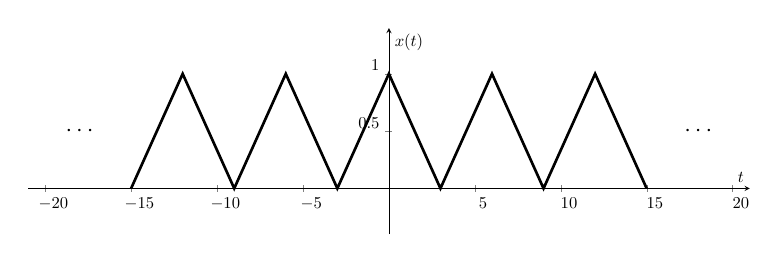
\begin{tikzpicture}[scale=0.6,transform shape]
    \begin{axis}[
        x=0.03\textwidth,y=0.2\textwidth,
    	axis y line=center,
    	axis x line=middle,
    	xlabel=$t$,ylabel=$x(t)$,
    	xmin=-21,xmax=21,
    	ymin=-0.4,ymax=1.4,
    	xticklabel style = {xshift=5},
    	yticklabel style = {yshift=5},
    	]
    	\addplot[
    	black,
    	ultra thick
    	] coordinates {
    	    (-15,0) (-12,1) 
    	    (-9,0) (-6,1)
    	    (-3,0) (0,1)
    	    (3,0) (6,1)
    	    (9,0) (12,1)
    	    (15,0)
    	};
    	\node at (18,0.5) {\Large $\cdots$} ;
    	\node at (-18,0.5) {\Large $\cdots$} ;
    \end{axis}
\end{tikzpicture}